\documentclass[final]{beamer}

\mode<presentation>{\usetheme{OIST}}

% Packages needed for the poster
\usepackage[orientation=portrait,size=a0,scale=1.4]{beamerposter}
\usepackage[english]{babel}
\usepackage[latin1]{inputenc}

% Style of equations
\usefonttheme[onlymath]{serif}
\boldmath

% Put images in the figures folder
\graphicspath{{figures/}}

% Add packages that you need
\usepackage{braket}
\usepackage{amsmath}

% Poster header anf footer
\title{\huge Non-adiabatic generation of NOON states \\ in a Tonks--Girardeau gas}
\author{\textbf{James Schloss}, Albert Benseny, J\'er\'emie Gillet, Jacob Swain and Thomas Busch}
\institute[OIST]{Quantum Systems Unit, OIST Graduate University, Okinawa, Japan \\ https://groups.oist.jp/qsu \hspace{120pt} james.schloss@oist.jp}
\date[Sep. 8th, 2009]{Sep. 8th, 2009}
\newcommand{\leftfooter}{Okinawa Institute of Science and Technology Graduate University}
\newcommand{\rightfooter}{james.schloss@oist.jp}

% Poster
\begin{document}
\begin{frame}
\begin{columns}[t]

% First  column
\begin{column}{.49\textwidth}

\begin{block}{Introduction}
  \begin{itemize}
    \item Quantum superposition states are difficult to generate experimentally. One example is the NOON state.
    \begin{itemize}
      \item The $\ket{N,0} + \ket{0,N}$ or ``NOON" state is a superposition state where all particles can be found in either one state or another.
      \item This state requires strong correlations between particles.
    \end{itemize}
    \item This project studies the following:
    \begin{itemize}
      \item The generation of NOON states in a ring of strongly correlated, \\ ultracold atoms through an adiabatic technique.
      \item The application of the Chopped RAndom Basis (CRAB) Optimal Control [1] along with Shortcuts to Adiabaticity (STA) techniques to generate NOON states non-adiabatically.
    \end{itemize}
  \end{itemize}
\end{block}

\vfill

\begin{block}{Rotating Ring Trap}
  \begin{itemize}
    \item Our system is a ring of strongly correlated ultracold atoms in the Tonks-Girardeau regime with the following properties:
    \begin{itemize}
      \item The bosons are fermionized.
      \item It is 1-dimensional with periodic boundaries.
      \item There is potential barrier that ``stirs" the trap.
    \end{itemize}
  \end{itemize}
  \centering
  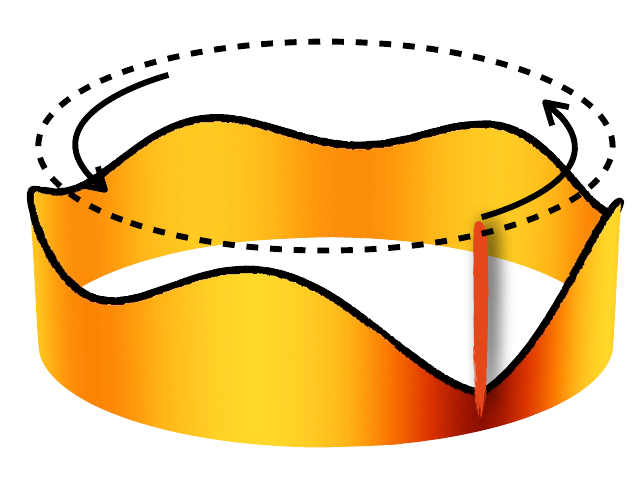
\includegraphics[width=0.4\linewidth]{figures/ring.png}
  \begin{itemize}
    \item We can model a system of $N$ atoms with a mass $M$ in a loop with a circumference of $L$ with the 1-dimensional Hamiltonian [2]
    $$\sum_{i=0} ^{N} \bigg[{\frac{\hbar}{2M}\bigg(-i\frac{\partial}{\partial x_i}-\Omega}\bigg)^2 + b\delta(x_i) +g \sum_{i<j} ^{N} \delta (x_i - x_j )\bigg],$$
    \item A single particle will rotate and form different rotational states, shown in the energy spectrum (below).
    \begin{itemize}
      \item With a barrier present, there are avoided crossings in the rotational states at integer values of $\pi$.
      \item NOON states are found at the positions of the avoided crossings
    \end{itemize}
  \end{itemize}
  \centering
  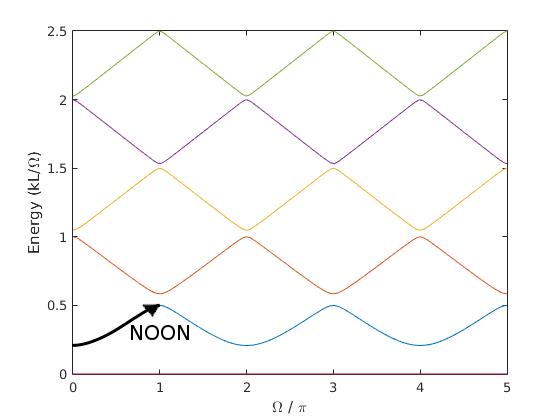
\includegraphics[width=0.7\linewidth]{figures/criss-cross_2}
  \vskip-1ex
\end{block}

\vfill

\begin{block}{CRAB Algorithm}
  \begin{itemize}
    \item The Chopped RAndom Basis (CRAB) Optimal Control technique changes a guess pulse [1]
    $$\Omega^{CRAB}_j(t) = \Omega^0_j(t)g_j(t)$$
    $\Omega^0_j$ is an initial guess we provide that is modified by $g_j(t)$, the function to be optimized
    $$g(t) = 1 + \frac{\sum^{N}_{n = 0}A_n\sin(\omega_nt)+B_n\cos(\omega_nt)}{\lambda(t)}$$
    Where $\lambda(t)$ is a function, chosen such that $\lambda(t) \rightarrow \infty$ for $t \rightarrow 0$ and $t \rightarrow T$. In our implementation, $$\lambda(t) = \frac{T^2}{4t(t-T)}$$
    \item This technique is performed continually with the Nelder--Mead, or ``downhill simplex," method to maximize the fidelity (or closeness) to the NOON state.
  \end{itemize}

\end{block}
\end{column}


% Second column
\begin{column}{.49\textwidth}

\begin{block}{STA techniques}
  \begin{itemize}
    \item STA techniques use semi-analytical shortcuts to speed up quantum adiabatic processes.
    \item Our technique initially raises a potential adiabatically and then rotates the system into the desired state.
    \item In contrast to optimal control, STA techniques have a lower numerical complexity, but have initially adiabatic steps.
  \end{itemize}
  \centering
  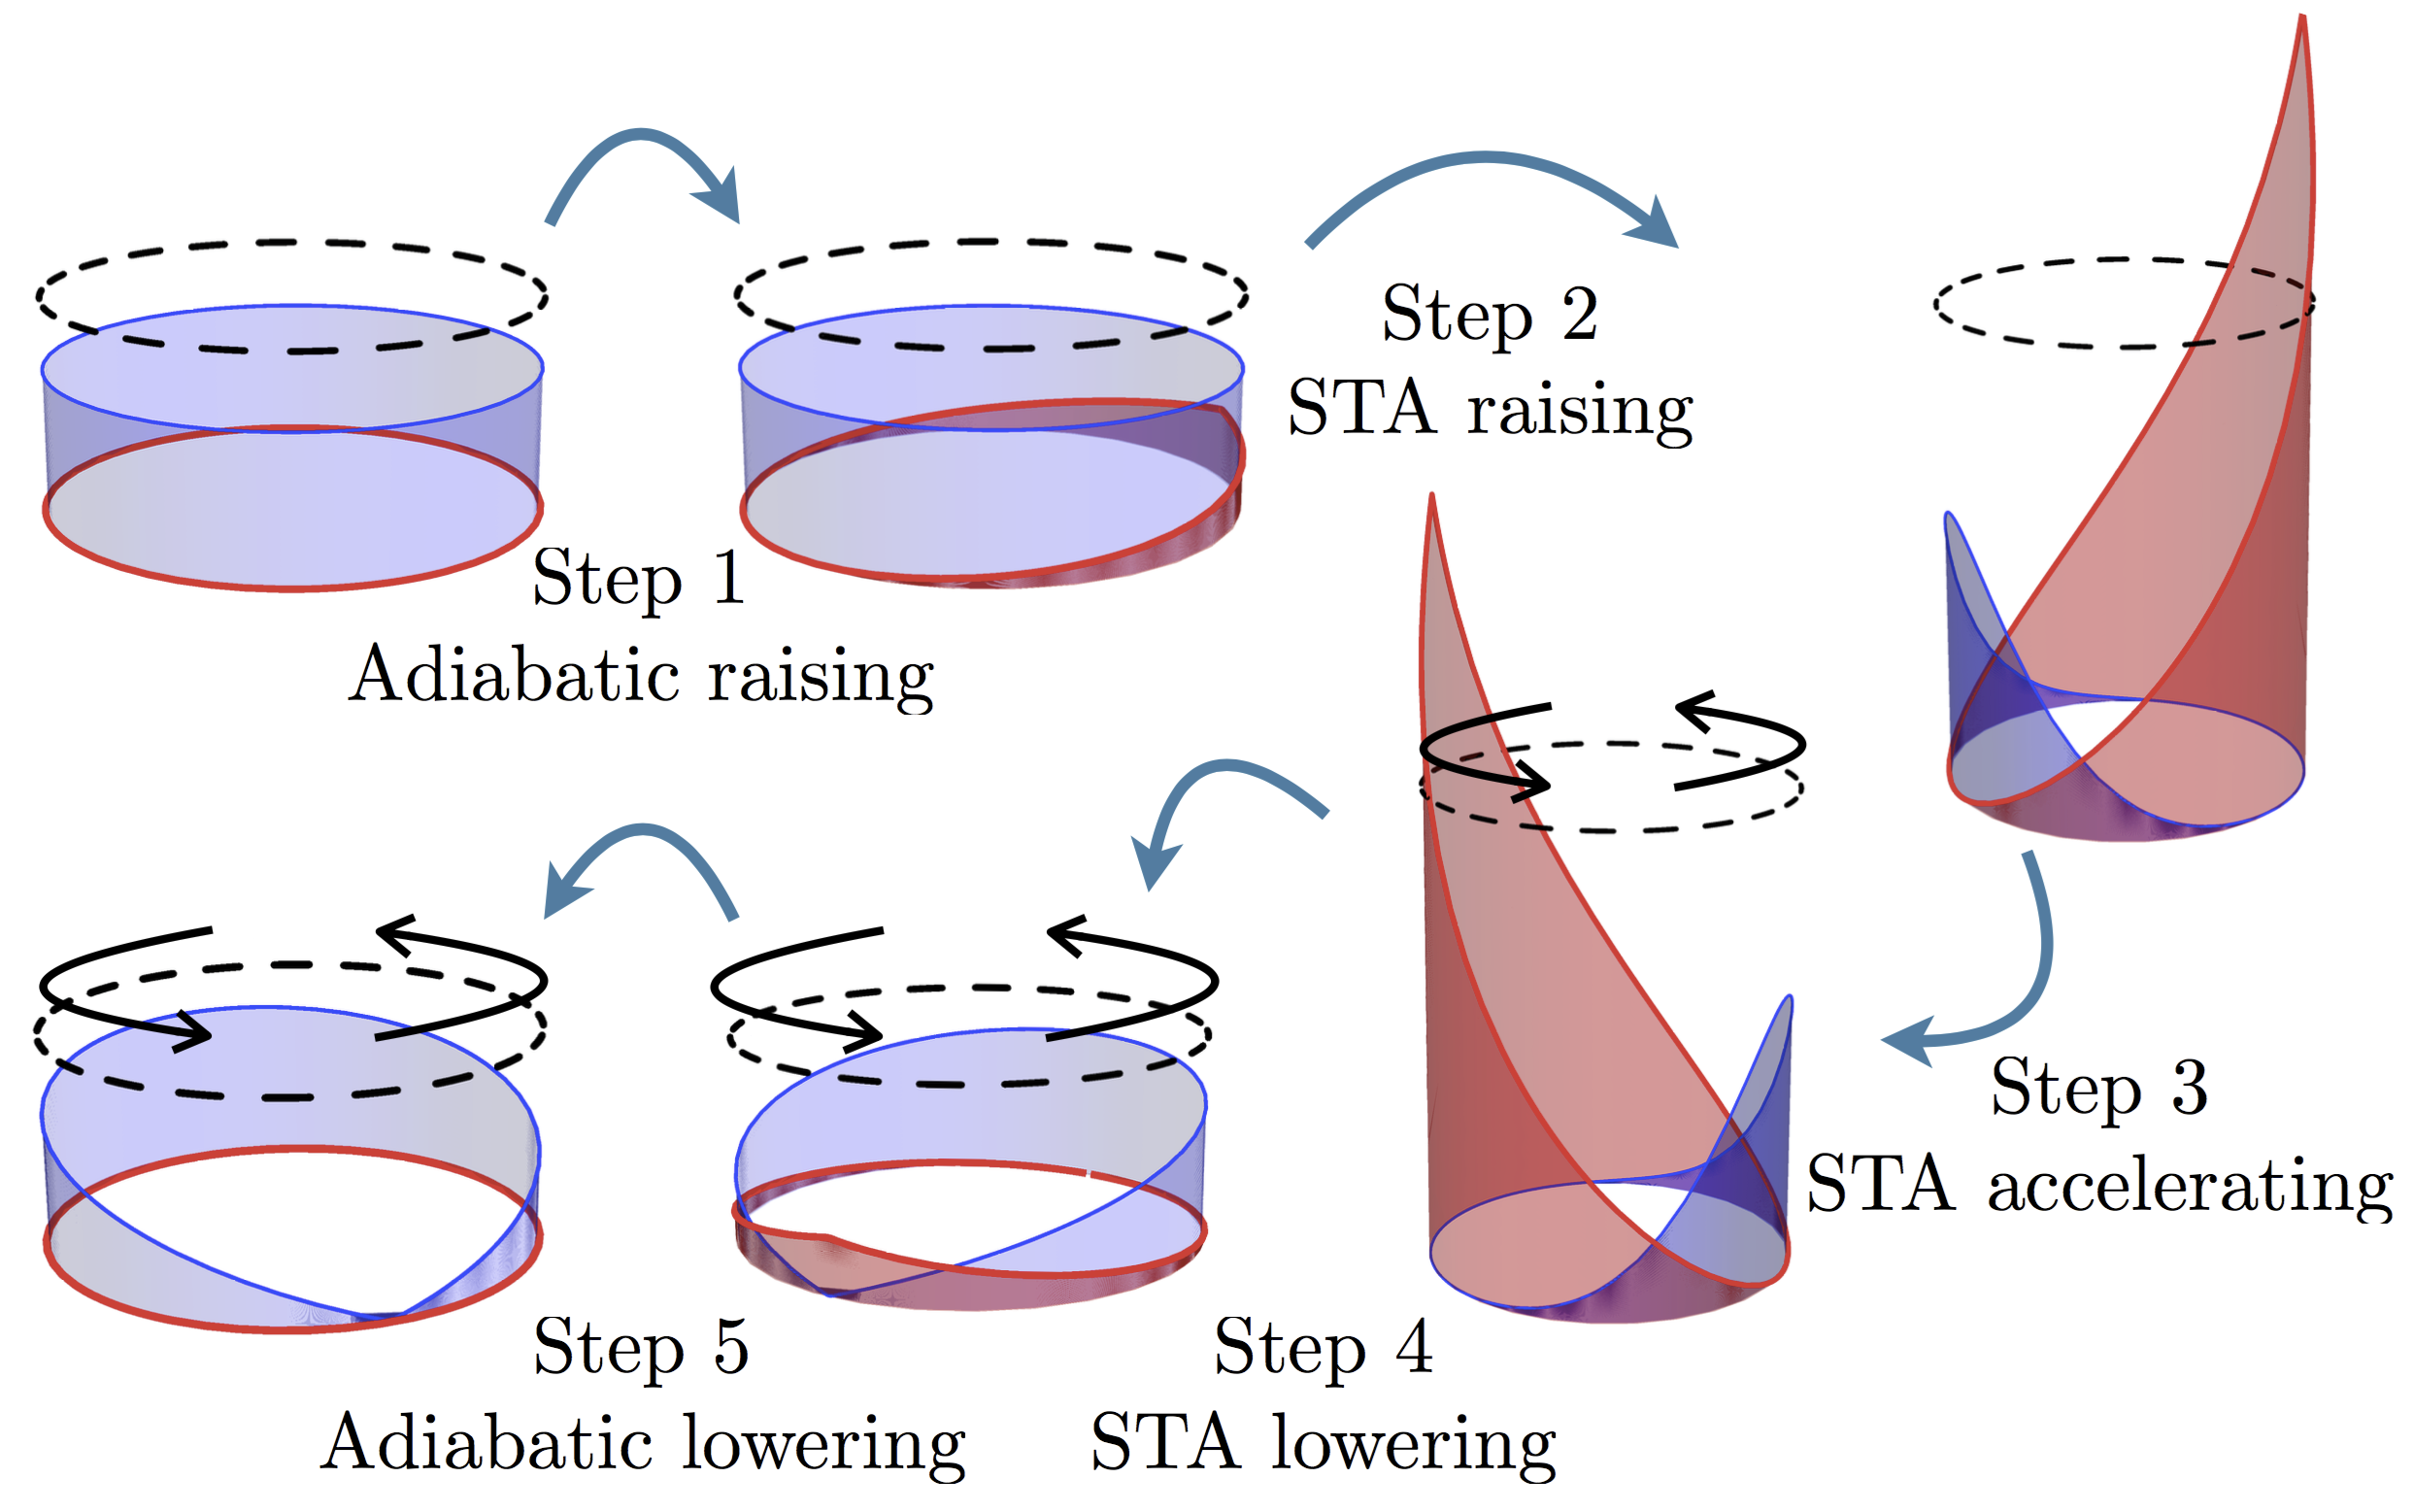
\includegraphics[width=0.85\linewidth]{STAscheme.png}
\end{block}

\vfill

\begin{block}{Results}
  \begin{itemize}
    \item With the CRAB algorithm, we found optimal rotational pulses at much shorter timescales than with STA techniques.
    \item It is also possible to manipulate the barrier height with the CRAB algorithm.
  \end{itemize}
  \centering
  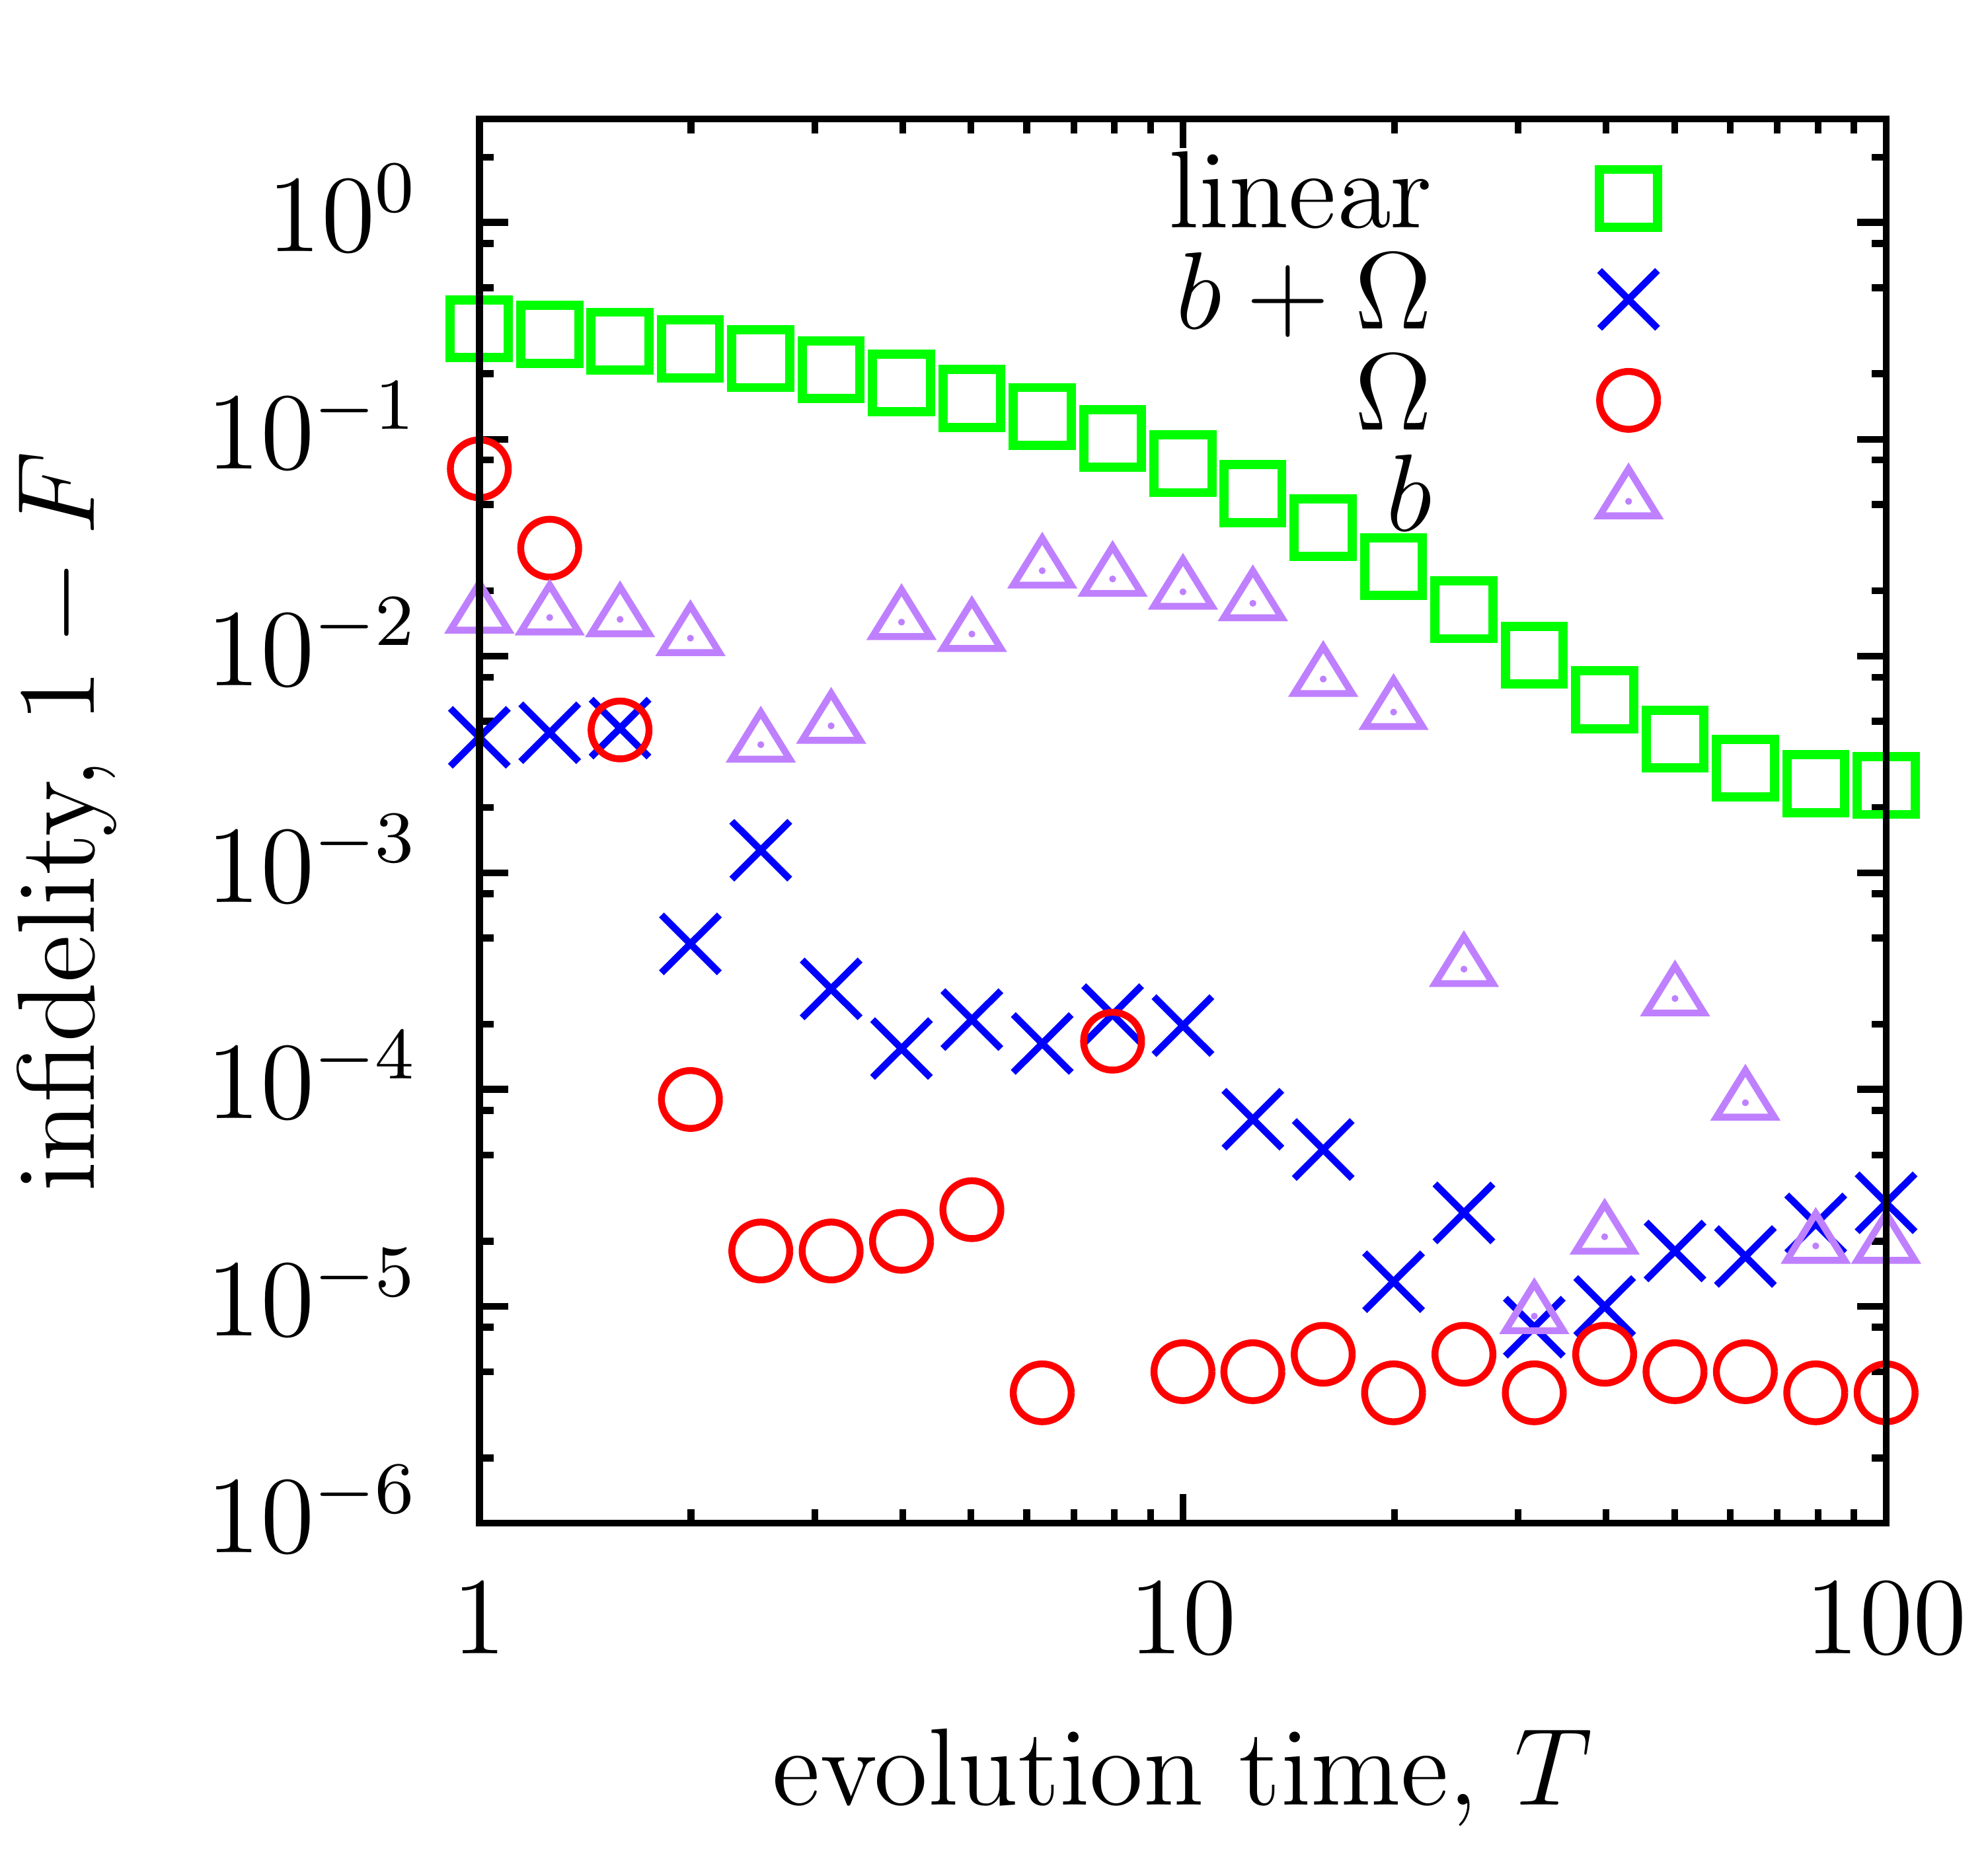
\includegraphics[width=0.5\linewidth]{final.png}
  \begin{itemize}
    \item With STA tecniques, we found high fidelities until $N = 15$ bosons for a harmonic trap $V_H$ and $N=21$ for a sinusoidal trap $V_S$.
  \end{itemize}
  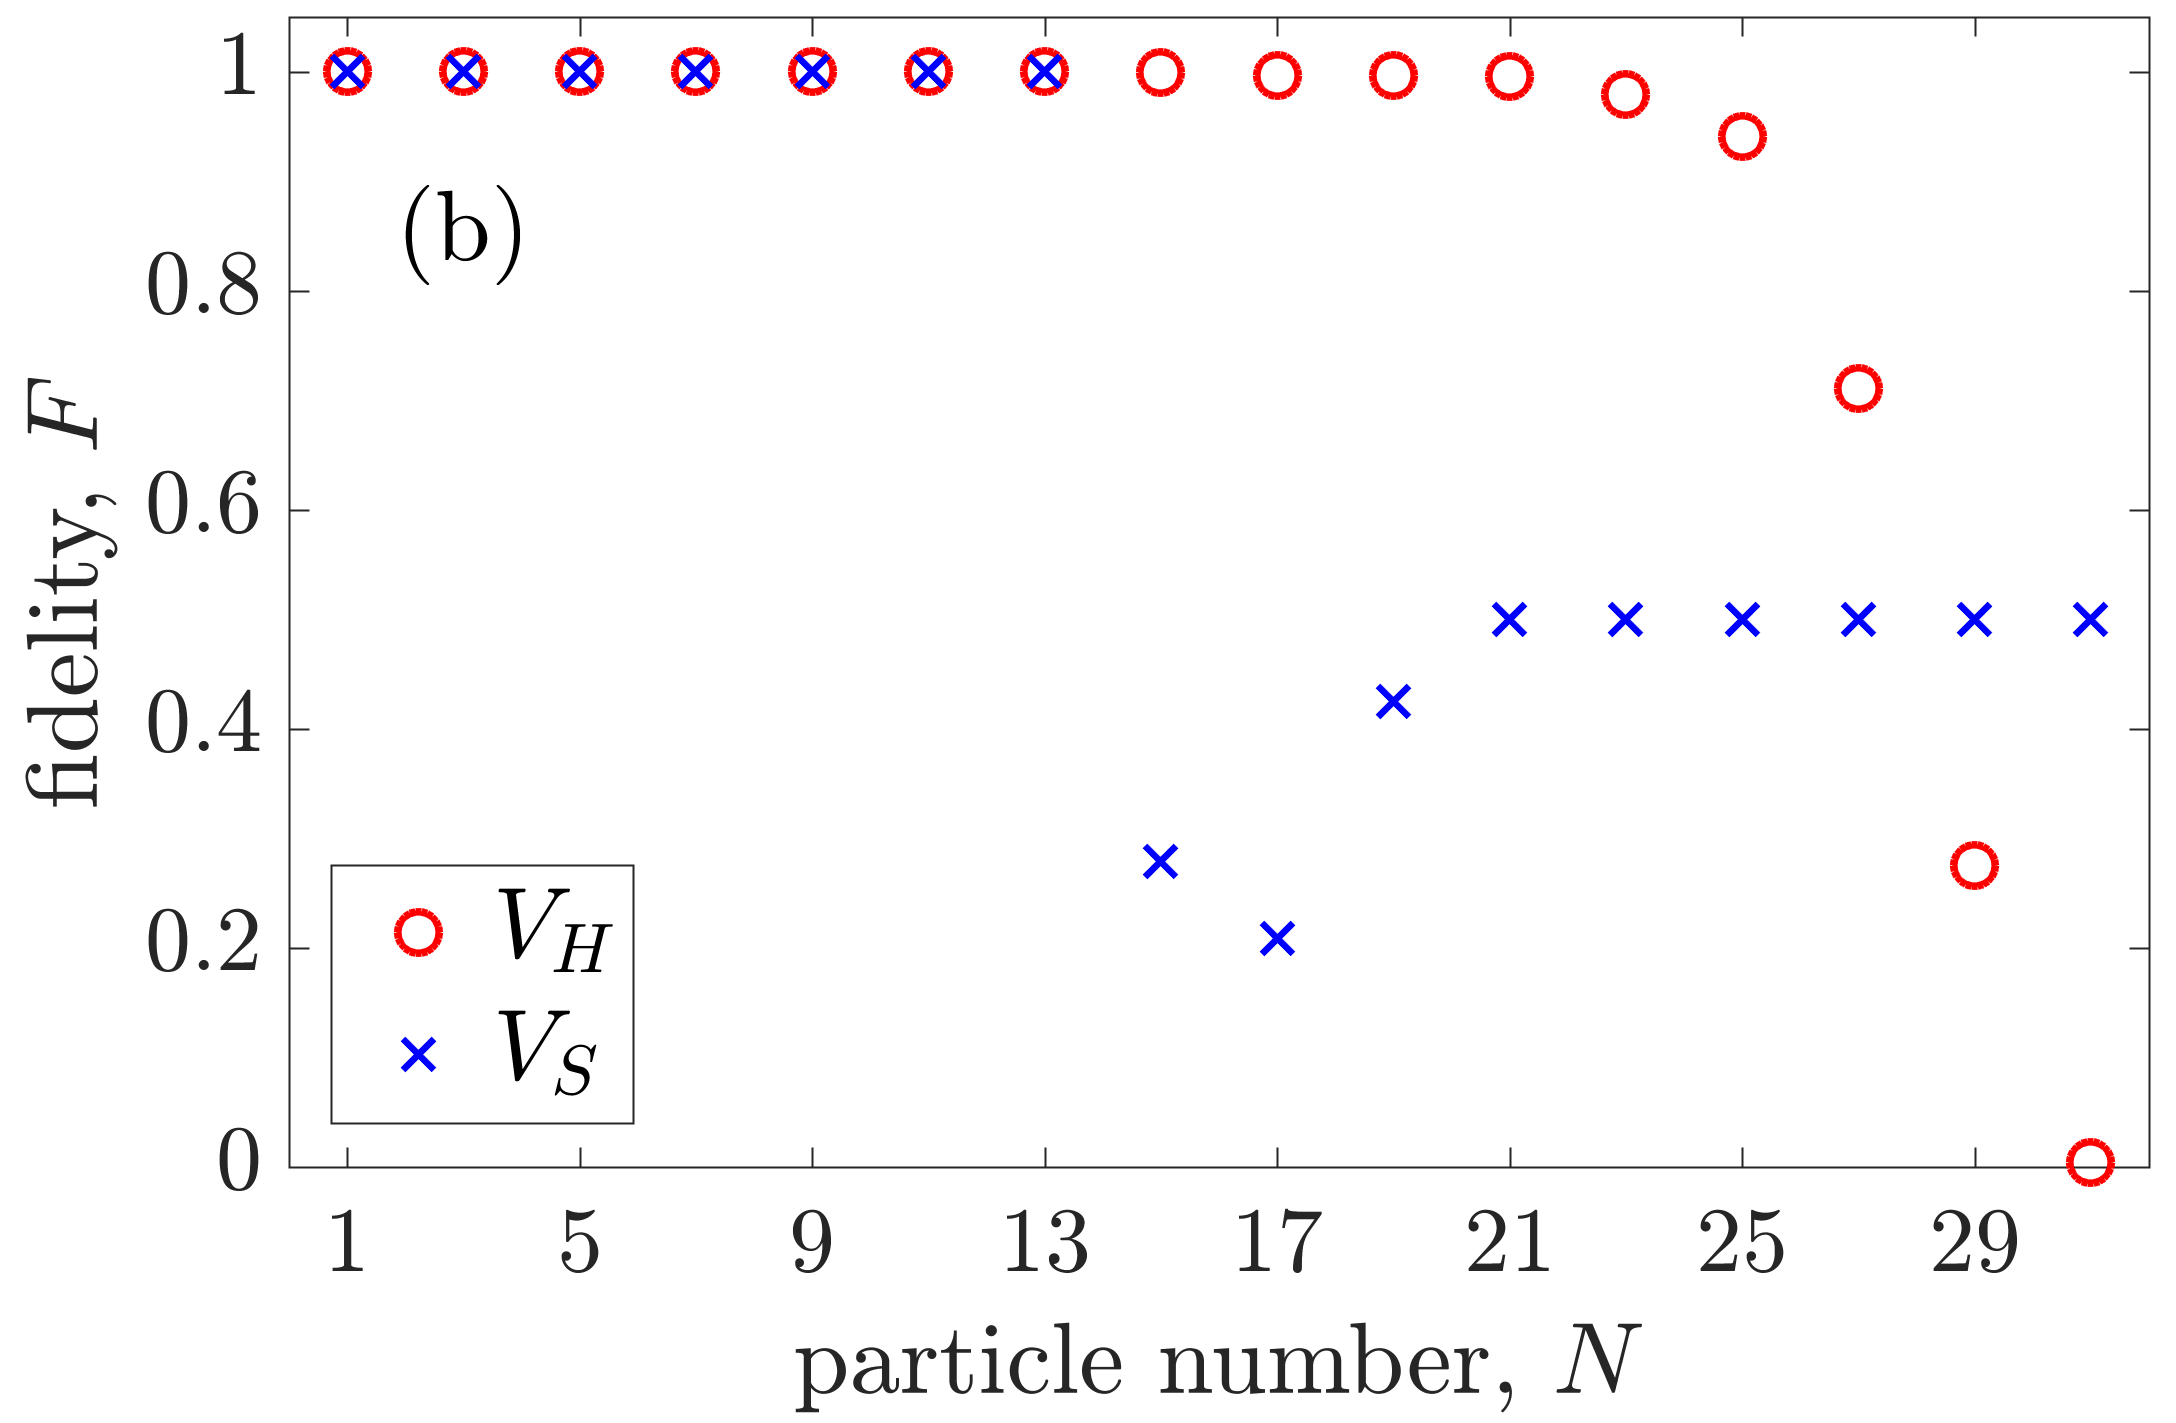
\includegraphics[width=0.6\linewidth]{fig7b.png}
\end{block}

\vfill

\begin{block}{Conclusions}
  We have shown:
  \begin{itemize}
    \item It is possible to manipulate either the rotation or barrier heght within a specified time regime to create NOON states on a rotating ring of strongly correlated ultracold atoms by using the CRAB optimal control technique.
    \item We may generate NOON states with STA in this system with up to $N=15$ bosons for a harmonic trap and $N=21$ for a sinusoidal trap.
  \end{itemize}
  These results have been published in [3].

  \hrulefill

  [1] T. Caneva, T. Calarco and S. Montangero, \textit{Phys. Rev. A}, 84:022326 \hspace*{3ex}(2011)

  [2] D. Hallwood, T. Ernst and J. Brand, \textit{Phys. Rev. A}, 82:063623 (2010)

  [3] J. Schloss, A. Benseny, J. Gillet, J. Swain and Th. Busch, \\ \hspace*{3ex}\textit{New J. of Phys.}, 18:035012 (2016)

\end{block}
\end{column}
\end{columns}
\end{frame}
\end{document}
